\documentclass[a4paper]{article}
\usepackage[margin=1in]{geometry} 
% \usepackage{ctex}
\usepackage{tabularx}
\usepackage{lipsum}
\usepackage{enumerate}
\usepackage{amsfonts}
\usepackage{multirow}
\usepackage{graphicx}

\begin{document}
\begin{titlepage}
    \title{\textbf{Lab Report: Investigating how the falling distance affects the speed of an object}}
    \author{Eric Zhou}
    \date{\today}
    \maketitle
    \tableofcontents
\end{titlepage}

\section{Introduction}

We have learned in physics that any falling object near earth has an acceleration of free fall $g$, whose value is about $9.8ms^{-2}$. This experiment is designed to testify that theory.

In this experiment, \textbf{falling distance} refers to the distance the object has travelled since it is released freely, provided no external force other than gravitational force. \textbf{Speed} is the rate of change of position, as is defined in physics.

Research question: \textbf{What is the relationship between the falling distance and the speed of an object that had been released freely and has fallen by that distance.}

\section{Background Knowledge}

People have not developed a systematic theory to explain the free fall until the 17th century. In ancient Greece, Aristotle proposed that the speed of a falling body would be proportional to its weight. That theory was widely accepted. Some objection was raised but it was not until Galileo dropped two objects of unequal mass from the Leaning Tower of Pisa that Aristotle's theory was completely proven wrong. It takes hundreds of years before people accept the new theory. Later, Newton discovered the Newton's Law of Motion, using mathematical way to fully explain the pheonomenon. In 1807, Thomas Young invented the concept of energy. That concept, although derived from Newton's Laws, provided a more simple explanation of the acceleration of free fall.

\section{Hypothesis and Reasoning}

If the release height is higher, the speed will be faster.

According to the conservation of energy, the gravitational potential energy released should be transfromed mainly into the kinetic energy of the object. That is to say,

$$mgh = {1\over 2} m v ^ 2$$

From which we can easily get 

$$v^2 = 2gh$$

indicating that $v^2$, the square of the falling speed should be directly proportional to $h$, the height. Since the density of the object is quite high, the effect of air resistance is considered negeligible.

\section{Experiment design}

\subsection{Variables}

\begin{itemize}
    \item Independent Variable: Height $h$($30cm,50cm,70cm,90cm,110cm$. measured by a metre rule)
    \item Dependent Variable: The time needed for the object to pass the photogate.
    \item Controlled Variables: The size, mass, material of the object, the temperature and humidity of the environment, etc. They are listed in Table 1.
\end{itemize}

\begin{table}[ht!]
    \centering
    \caption[short]{Controlled Variables}
    \begin{tabularx}{0.8 \textwidth}{|X|X|X|X|}
    \hline
    Controlled Variable          & Specific Control Variable Value      & Reason to control                                                    & Method to control                                  \\
    \hline
    Size and shape of the object & Sphere, diametre = $1.82\pm 0.005cm$ & Might affect the time taken to completely pass through the photogate & Use the same object                                \\
    \hline
    Temperature                  & Local temperature. $31^oC\pm 1^oC$   & Might affect the air resistance.                                     & Complete the experiment during a short time period \\
    \hline
    Altitude                     & Local elevation. Less than $150m$    & Might affect the gravitational acceleration.                         & Complete the experiment in one place              \\
    \hline
    \end{tabularx}
\end{table}

\subsection{Materials}

\begin{itemize}
    \item 2 $\times$ iron stand
    \item 1 $\times$ plumb line (about $120$ cm long)
    \item 1 $\times$ metal ball (diametre $d \approx 2cm$)
    \item 1 $\times$ photogate
    \item 1 $\times$ electromagnet
    \item 1 $\times$ meter rule
    \item 1 $\times$ soft cushion
    \item 1 $\times$ vernier caliper
\end{itemize}

\subsection{Set up diagram}

\begin{figure}[h!]
    \centering
    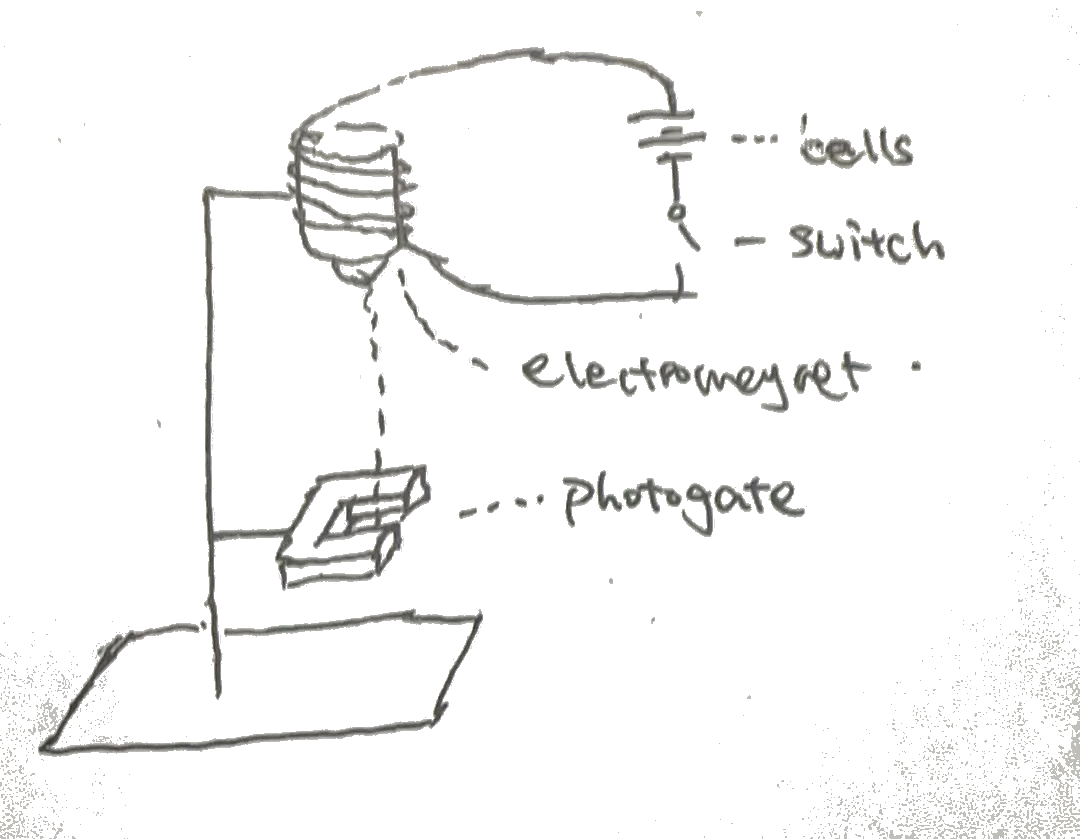
\includegraphics[width = 0.6\textwidth]{setup.png}
\end{figure}

\subsection{Method}

\begin{enumerate}[1.]
    \item Use the vernier caliper to obtain the diametre of the metal ball, $d$.
    \item Attach the photogate to the lower iron stand.
    \item Attach the electromagnet to the higher iron stand.
    \item Adjust the iron stands to make the height difference to be $h = 30 cm$.
    \item Close the circuit of the electromagnet. Attach the metal ball to it.
    \item Break the circuit and take down the reading $t_1$ on the photogate.
    \item Repeat Step 6 twice to take down $t_2$ and $t_3$.
    \item Repeat Steps 2\~7 with $h = 50cm,70cm,90cm,110cm$.
\end{enumerate}

\subsection{Risk Assessment}

This experiment is relatively safe with little potential hazard. It is still needed to pay attention to his feet's position to avoid being hit by the ball, though.

\section{Results}
    \subsection{Raw data}
    \begin{table}[ht!]\centering
        \caption{Raw Data}
        \begin{tabular}{|l|l|lll|}
        \hline
        \multirow{2}{*}{Experiment} & \multirow{2}{*}{Height($h$)/cm} & \multicolumn{3}{l|}{Time to pass photo gate($t$)/ms}                  \\ \cline{3-5} 
                                    &                                 & \multicolumn{1}{l|}{Trial 1} & \multicolumn{1}{l|}{Trial 2} & Trial 3 \\ \hline
        1                           & $30 \pm 0.05$                   & \multicolumn{1}{l|}{7.00}    & \multicolumn{1}{l|}{7.07}    & 7.09    \\ \hline
        2                           & $50 \pm 0.05$                   & \multicolumn{1}{l|}{5.28}    & \multicolumn{1}{l|}{5.38}    & 5.00    \\ \hline
        3                           & $70 \pm 0.05$                   & \multicolumn{1}{l|}{4.29}    & \multicolumn{1}{l|}{4.24}    & 4.25    \\ \hline
        4                           & $90 \pm 0.05$                   & \multicolumn{1}{l|}{4.10}    & \multicolumn{1}{l|}{4.10}    & 4.13    \\ \hline
        5                           & $110 \pm 0.05$                  & \multicolumn{1}{l|}{3.31}    & \multicolumn{1}{l|}{3.71}    & 3.51    \\ \hline
        \end{tabular}
    \end{table}
    % [0.07505553499465135, 0.05813776741499453, 0.049135381491199545, 0.043333333333333335, 0.03919647479510927]
    \subsection{Processed data}
    
    \begin{table}[ht!]\centering
        \caption{Processed Data}
        \begin{tabular}{|l|l|l|l|l|}
        \hline
        Experiment & Average Time $\bar{t}$ (ms) & Percentage Error & Speed & Percentage Error \\ \hline
        1          & 7.05                        & 1.28\%            & 2.58  & 2.05\%            \\ \hline
        2          & 5.22                        & 7.28\%            & 3.48  & 7.55\%            \\ \hline
        3          & 4.26                        & 1.17\%            & 4.27  & 0.44\%            \\ \hline
        4          & 4.11                        & 0.73\%            & 4.43  & 1.00\%            \\ \hline
        5          & 3.51                        & 11.4\%            & 5.19  & 11.7\%            \\ \hline
        \end{tabular}
    \end{table}
    \begin{figure}[h!]
        \centering
        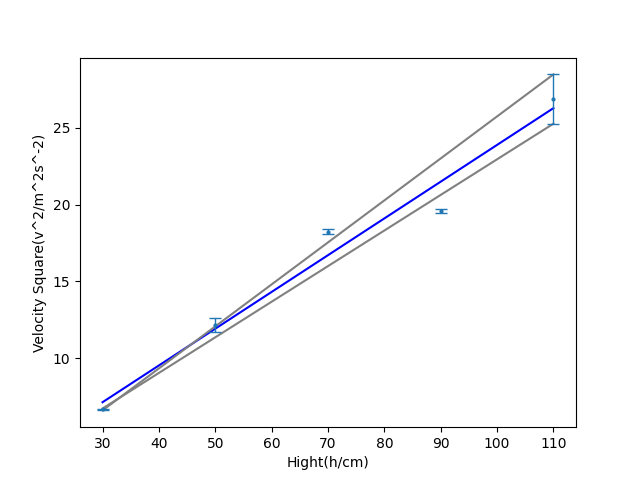
\includegraphics[width = 0.5\textwidth]{Figure_1.png}
    \end{figure}

    \subsection{Sample working}
        To calculate the average time taken to completely pass through the photogate ($\bar{t}$):

        $$\bar{t} = {{t_1+t_2+t_3}\over 3} = {{7.00+7.07+7.09} \over 3} s \approx 7.05 ms$$.

        The speed passing the photogate ($v$)

        $$v = {d \over \bar{t}} = {1.82cm \over 7.05ms} \approx 2.58 m/s$$

\section{Discussion and conclusion}

Our diagram suggests

\begin{itemize}
    \item A slope of $0.240$.
    \item A y-intercept of $-0.0556$.
\end{itemize}

From which we can derive $g = {{v^2}\over{2h}} = {2\over{0.240}}\approx 8.3ms^{-2}$. This is close to $9.8ms^{-2}$.

The y-intercept is expected to be zero, but $-0.0556$ is found.

Considering the small error, the results support our initial hypothesis. That is, higher the releasing height, faster the speed. The square of the speed should be proportional to the height.

\section{Evaluation}

\begin{table}[!ht]
    \centering
    \caption{Evaluation }\label{tab:dummy-1}
    {
      \begin{tabularx}{0.8\textwidth} {|X|X|X|}
        \hline
        Limitation & Significancy & Improvement \\
        \hline
        It's difficult to make the height difference exactly the same as expected. & Might lead to inaccurate $h$ and hence inaccurate $t$  & Choose a better iron stand.\\
        \hline
        The metal ball may not fall exactly through the photogate as expected. & No reading, or a too small reading if the center of the object is a little away from the center of the photogate. & Use a glass tube too correct the falling route. \\
        \hline
        Might be affacted by air resistance. & Lenghthen the time needed to pass the photogate. & Use an object with a higher density.\\
        \hline
      \end{tabularx}
    }
  \end{table}

\end{document}